\section{Foundations}
\label{sec:foundations}

We build the theory from a single starting point: a finite alphabet. Every externalized piece of knowledge is a finite string; structured knowledge is a finite sequence of key-value pairs of strings. From this minimal assumption we construct hash identifiers and a reference structure, arriving at the \emph{signature} $\Sigma = (S, h_{\mathrm{id}})$. Records in a signature are graded by the number of other records they reference, yielding a \emph{semantic simplicial complex} $\Delta(\Sigma) = \bigsqcup_{k \geq 0} \Delta_k$, on which the algebraic topology of \S\ref{sec:topology} operates. The geometric structure (semantic embeddings, metrics) is introduced in \S\ref{sec:semantics}.

\subsection{Alphabet and String Space}

\begin{definition}[Alphabet]
\label{def:alphabet}
An \emph{alphabet} is a finite set $A$. We impose no structure on $A$ beyond finiteness; it may be the set of Unicode code points, ASCII characters, or any other finite encoding.
\end{definition}

\begin{definition}[Monoid]
\label{def:monoid}
A \emph{monoid} is a triple $(M, \cdot, e)$ where $M$ is a set, $\cdot : M \times M \to M$ is an associative binary operation, and $e \in M$ is an identity element: $e \cdot m = m \cdot e = m$ for all $m \in M$.
\end{definition}

\begin{definition}[String space]
\label{def:string-space}
The \emph{string space} $A^*$ is the free monoid on $A$: the set of all finite sequences of elements of $A$, with concatenation as the monoid operation and the empty sequence $\varepsilon$ as identity.
\end{definition}

Every \LaTeX\ file, every Lean source, every JSON document, and every natural-language paragraph is an element of $A^*$ for an appropriate choice of $A$ (e.g., $A_{\mathrm{ASCII}}$ with $|A| = 128$, or the full Unicode code point set).

\begin{theorem}[Universal property of $A^*$]
\label{thm:free-monoid}
For any monoid $(M, \cdot, e)$ and any function $f : A \to M$, there exists a unique monoid homomorphism $\bar{f} : A^* \to M$ extending $f$.
\end{theorem}

In Lean~4, $A^*$ is \texttt{FreeMonoid} in Mathlib, and the universal property is \texttt{FreeMonoid.lift}, a corollary of the adjunction $\mathrm{Free} \dashv U$ between the free monoid functor and the forgetful functor. The universal property guarantees that any structure-preserving interpretation of the alphabet extends uniquely to all strings; this is the algebraic foundation of parsing.

\subsection{Record, Parsing, and Signature}

\begin{definition}[Record space]
\label{def:record-space}
A \emph{record} is a finite sequence of key-value pairs, where both keys and values are strings:
\[
  R = (A^* \times A^*)^*.
\]
A record $r = ((k_1, v_1), \ldots, (k_n, v_n)) \in R$ assigns to each key $k_i$ a value $v_i$. Keys may repeat; the order of pairs is significant.
\end{definition}

\begin{definition}[Parsing]
\label{def:parsing}
Let $\mathcal{P}_{\mathrm{fin}}(R)$ denote the set of finite subsets of $R$:
\[
\mathcal{P}_{\mathrm{fin}}(R) = \{ S \subseteq R \mid |S| < \infty \}.
\]
A \emph{parsing procedure} is a function $P : A^* \to \mathcal{P}_{\mathrm{fin}}(R)$ that maps a string to a finite set of records. Different parsing procedures extract different structures from the same string; we distinguish them by subscripts ($P_{\mathrm{compiler}}$, $P_{\mathrm{LLM}}$, etc.).
\end{definition}

\begin{example}
Consider the Lean source file $s \in A^*$:
\begin{minted}[fontsize=\scriptsize]{lean4}
theorem length_append (l1 l2 : List a) :
    (l1 ++ l2).length = l1.length + l2.length := by
  induction l1 <;> simp [*]
\end{minted}
\noindent Three parsers extract different sets of records from the same string:
\begin{itemize}
\item $P_{\mathrm{compiler}}(s)$: the Lean~4 compiler reads \texttt{.ilean} artifacts and produces one record per declaration. Writing each record as an element of $R = (A^* \times A^*)^*$:
\begin{align*}
r_1 &= ((\texttt{name},\; \texttt{length\_append}),\; (\texttt{sort},\; \texttt{theorem}),\; (\texttt{stmt},\; \ldots\,)) \in R, \\
r_2 &= ((\texttt{name},\; \texttt{List.length}),\; (\texttt{sort},\; \texttt{definition})) \in R, \\
r_3 &= ((\texttt{name},\; \texttt{List.append}),\; (\texttt{sort},\; \texttt{definition})) \in R, \\
r_4 &= ((\texttt{name},\; \texttt{Nat.add}),\; (\texttt{sort},\; \texttt{definition})) \in R.
\end{align*}
Thus $P_{\mathrm{compiler}}(s) = \{r_1, r_2, r_3, r_4\} \in \mathcal{P}_{\mathrm{fin}}(R)$.

\item $P_{\mathrm{LLM}}(s)$: a language model reads the same file as natural language and extracts records for each mathematical concept:
\[
P_{\mathrm{LLM}}(s) = \bigl\{\,
((\texttt{name},\; \texttt{list concatenation}),\; (\texttt{sort},\; \texttt{concept})),\;\ldots
\,\bigr\} \in \mathcal{P}_{\mathrm{fin}}(R).
\]

\item $P_{\mathrm{AST}}(s)$: a syntax-level parser extracts the abstract syntax tree, producing records for each node:
\[
P_{\mathrm{AST}}(s) = \bigl\{\,
((\texttt{name},\; \texttt{length\_append}),\; (\texttt{sort},\; \texttt{theorem})),\;\ldots
\,\bigr\} \in \mathcal{P}_{\mathrm{fin}}(R).
\]
\end{itemize}
\noindent In general $P_{\mathrm{compiler}}(s) \neq P_{\mathrm{LLM}}(s) \neq P_{\mathrm{AST}}(s)$: different parsers extract different records from the same string. The framework is indifferent to domain; the same construction applies to Python modules, legal statutes, or biological databases.
\end{example}

\begin{definition}[Identity hash]
\label{def:identity-hash}
An \emph{identity hash} is a function $h_{\mathrm{id}} : H^* \times R \to H$ that maps a vertex list and a record to an identifier in $H$ (in practice, $H = \{0,\ldots,9,\texttt{a},\ldots,\texttt{f}\}^{12}$, the set of 12-character hexadecimal strings). The hash is computed from the concatenation of the serialized vertex list $\texttt{ref}$ and the essential part of $\texttt{record}$:
\[
h_{\mathrm{id}}(\texttt{ref},\; \texttt{record}) = \texttt{SHA256}\bigl(\texttt{serialize}(\texttt{ref}) \;\|\; \texttt{serialize}(\texttt{record}_{\mathrm{ess}})\bigr)[:12].
\]
Two simplices are considered identical if and only if they have the same vertex list and the same essential content.
\end{definition}

The identity hash is a content-addressing mechanism~\cite{Benet2014}: a simplex's identity is determined by \emph{what it connects} ($\texttt{ref}$) and \emph{what it says} ($\texttt{record}$), not by its location. This is the same principle underlying Git commits and IPFS~\cite{Benet2014}.

\begin{example}
For a 0-simplex (vertex):
\begin{minted}[fontsize=\scriptsize]{python}
ref    = '["a1b2c3"]'
record = '{"name":"Nat.add_comm","sort":"theorem","stmt":"..."}'
h_id   = sha256(ref + record).hexdigest()[:12]  # "a1b2c3"
\end{minted}
\noindent The 0-simplex's $\texttt{ref}$ contains its own hash, so the definition is self-referential: $h_{\mathrm{id}}$ is the unique fixed point of $h \mapsto \texttt{SHA256}([h] \| \texttt{record})[:12]$.

For a 1-simplex (edge) connecting two vertices:
\begin{minted}[fontsize=\scriptsize]{python}
ref    = '["a1b2c3","b2c3d4"]'
record = '{"sort":"uses","weight":"0.9"}'
h_id   = sha256(ref + record).hexdigest()[:12]  # "x7y8z9"
\end{minted}
\noindent The same two vertices with different $\texttt{record}$ produce a different hash---they are distinct 1-simplices. The same $\texttt{record}$ with different vertices also produces a different hash. Collision probability is $< 2^{-48}$ per pair, negligible for knowledge bases with $n < 10^6$ simplices.
\end{example}


\begin{definition}[Signature]
\label{def:signature}
A \emph{signature} is a pair $\Sigma = (S, h_{\mathrm{id}})$ where $S$ is a finite set of records and $h_{\mathrm{id}} : S \hookrightarrow H$ is an injective identity hash. Since $h_{\mathrm{id}}$ is injective, it induces a dictionary structure: each record $r \in S$ is uniquely indexed by its hash $h_{\mathrm{id}}(r)$.
\end{definition}

\subsection{Semantic Simplicial Complex}

\begin{definition}[Semantic simplex]
\label{def:semantic-simplex}
Let $\Sigma = (S, h_{\mathrm{id}})$ be a signature. A \emph{semantic simplex} is a triple $(\texttt{hash},\; \texttt{ref},\; \texttt{record})$ where:
\begin{itemize}
\item $\texttt{hash} \in H$ is the identity hash, generated by $h_{\mathrm{id}}$ from $\texttt{ref}$ and the essential part of $\texttt{record}$.
\item $\texttt{ref} = [v_0, v_1, \ldots, v_k]$ is an ordered list of hashes in $H$, called the \emph{vertex list}.
\item $\texttt{record} \in (A^* \times A^*)^*$ is the \emph{semantic content}: an open collection of key-value pairs.
\end{itemize}
The \emph{dimension} of the simplex is
\[
\dim(\sigma) = |\texttt{ref}| - 1.
\]
A 0-simplex (vertex) has $\texttt{ref} = [v_0]$ where $v_0$ is its own hash---it is its own sole vertex. A $k$-simplex ($k \geq 1$) has $\texttt{ref} = [v_0, \ldots, v_k]$ referencing $k + 1$ vertices. The ordering of $\texttt{ref}$ determines the face maps and the signs in $\partial$.

We write $\Delta_k = \{ \sigma \in S \mid |\texttt{ref}(\sigma)| = k + 1 \}$ for the set of all $k$-semantic simplices.
\end{definition}

\begin{figure}[ht]
\centering
\begin{tabular}{|l|c|c|c|}
\hline
& $k = 0$ (vertex) & $k = 1$ (edge) & $k = 2$ (face) \\
\hline
% --- Row 1: geometry ---
\textbf{Simplex}
&
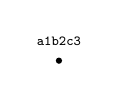
\begin{tikzpicture}[baseline=-5pt,
  v/.style={circle, fill, inner sep=0.8pt}]
\node[v] (p) at (0,0) {};
\node[font=\tiny, above=2pt] at (p) {\texttt{a1b2c3}};
\end{tikzpicture}
&
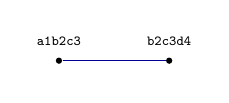
\begin{tikzpicture}[baseline=-5pt,
  v/.style={circle, fill, inner sep=0.8pt}]
\node[v] (a) at (0,0) {};
\node[v] (b) at (1.4,0) {};
\draw[very thin, blue!60!black] (a)--(b);
\node[font=\tiny, above=2pt] at (a) {\texttt{a1b2c3}};
\node[font=\tiny, above=2pt] at (b) {\texttt{b2c3d4}};
\end{tikzpicture}
&
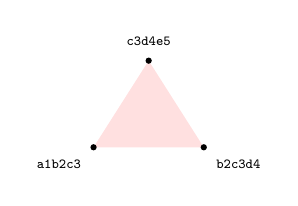
\begin{tikzpicture}[baseline=-5pt,
  v/.style={circle, fill, inner sep=0.8pt}]
\coordinate (a) at (0,0);
\coordinate (b) at (1.4,0);
\coordinate (c) at (0.7,1.1);
\fill[red!12] (a)--(b)--(c)--cycle;
\node[v] at (a) {};
\node[v] at (b) {};
\node[v] at (c) {};
\node[font=\tiny, below left=1pt] at (a) {\texttt{a1b2c3}};
\node[font=\tiny, below right=1pt] at (b) {\texttt{b2c3d4}};
\node[font=\tiny, above=2pt] at (c) {\texttt{c3d4e5}};
\end{tikzpicture}
\\
\hline
% --- Row 2: h_id ---
$h_{\mathrm{id}}$
&
\texttt{\scriptsize a1b2c3}
&
\textcolor{blue!60!black}{\texttt{\scriptsize x7y8z9}}
&
\textcolor{red!40!black}{\texttt{\scriptsize q1r2s3}}
\\
\hline
% --- Row 3: JSON ---
\texttt{ssc.json}
&
\begin{minipage}[t]{0.25\textwidth}
\begin{minted}[fontsize=\tiny,frame=none,bgcolor=gray!5]{json}
"a1b2c3": {
 "ref": ["a1b2c3"],
 "record": {
  "name": "Nat.add_comm",
  "sort": "theorem",
  "stmt": "..."
 }
}
\end{minted}
\end{minipage}
&
\begin{minipage}[t]{0.25\textwidth}
\begin{minted}[fontsize=\tiny,frame=none,bgcolor=gray!5]{json}
"x7y8z9": {
 "ref": ["a1b2c3",
         "b2c3d4"],
 "record": {
  "sort": "uses",
  "weight": "0.9"
 }
}
\end{minted}
\end{minipage}
&
\begin{minipage}[t]{0.25\textwidth}
\begin{minted}[fontsize=\tiny,frame=none,bgcolor=gray!5]{json}
"q1r2s3": {
 "ref": ["a1b2c3",
         "b2c3d4",
         "c3d4e5"],
 "record": {
  "sort": "joint_step",
  "method": "apply"
 }
}
\end{minted}
\end{minipage}
\\
\hline
\end{tabular}
\caption{Semantic simplices of dimension $0$, $1$, $2$. Top: geometric representation with vertex $h_{\mathrm{id}}$'s (blue). Middle: dimension and simplex $h_{\mathrm{id}}$. Bottom: \texttt{ssc.json} storage format. Each simplex is a triple $(\texttt{hash}, \texttt{ref}, \texttt{record})$; the vertex list $\texttt{ref}$ has length $k+1$.}
\label{fig:simplices}
\end{figure}

\begin{definition}[Semantic simplicial complex]
\label{def:semantic-complex}
The \emph{semantic simplicial complex} is the graded set
\[
\Delta(\Sigma) = \bigsqcup_{k \geq 0} \Delta_k
\]
where $\Delta_k = \{ \sigma \in S \mid |\texttt{ref}(\sigma)| = k + 1 \}$. The index $k$ is the dimension: $\Delta_0$ contains all vertices, $\Delta_1$ all edges, $\Delta_2$ all faces, and so on.
\end{definition}

\begin{figure}[ht]
\centering
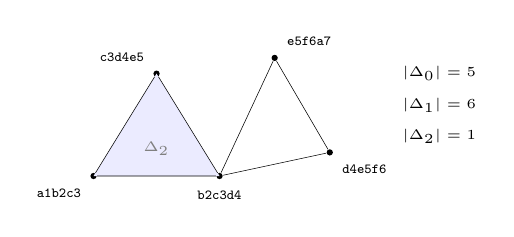
\begin{tikzpicture}[
  v/.style={circle, fill, inner sep=0.8pt},
  lbl/.style={font=\tiny}
]
\node[v] (A) at (0, 0) {};
\node[v] (B) at (1.6, 0) {};
\node[v] (C) at (0.8, 1.3) {};
\node[v] (D) at (3.0, 0.3) {};
\node[v] (E) at (2.3, 1.5) {};

\node[lbl, below left=1pt] at (A) {\texttt{a1b2c3}};
\node[lbl, below=2pt] at (B) {\texttt{b2c3d4}};
\node[lbl, above left=1pt] at (C) {\texttt{c3d4e5}};
\node[lbl, below right=1pt] at (D) {\texttt{d4e5f6}};
\node[lbl, above right=1pt] at (E) {\texttt{e5f6a7}};

\fill[blue!8] (A.center) -- (B.center) -- (C.center) -- cycle;
\draw[very thin] (A)--(B) (B)--(C) (A)--(C);
\draw[very thin] (B)--(D) (D)--(E) (B)--(E);

\node[font=\tiny, gray] at (0.8, 0.35) {$\Delta_2$};

\node[font=\tiny, anchor=west] at (3.8, 1.3) {$|\Delta_0| = 5$};
\node[font=\tiny, anchor=west] at (3.8, 0.9) {$|\Delta_1| = 6$};
\node[font=\tiny, anchor=west] at (3.8, 0.5) {$|\Delta_2| = 1$};
\end{tikzpicture}
\caption{A semantic simplicial complex $\Delta(\Sigma)$ with five vertices, six edges, and one filled face (the triangle $[v_0, v_1, v_2]$). The triangle $[v_1, v_3, v_4]$ is \emph{not} filled: the three edges exist but no 2-simplex with $\texttt{ref} = [v_1, v_3, v_4]$ is in $S$.}
\label{fig:complex}
\end{figure}

\begin{definition}[Face maps]
\label{def:face-maps}
For a $k$-simplex $\sigma$ with $\texttt{ref} = [v_0, \ldots, v_k]$, the \emph{$i$-th face map} is
\[
d_i(\sigma) = [v_0, \ldots, \hat{v}_i, \ldots, v_k], \qquad 0 \leq i \leq k,
\]
where $\hat{v}_i$ denotes omission of the $i$-th entry. The result is a vertex list of length $k$; the corresponding $(k-1)$-simplex may or may not exist in $S$.
\end{definition}

\begin{proposition}[Simplicial identity]
\label{prop:simplicial-identity}
The face maps satisfy
\[
d_i \circ d_j = d_{j-1} \circ d_i \quad \text{for } i < j.
\]
\end{proposition}

\begin{proof}
Removing $v_j$ first and then $v_i$ ($i < j$): after removing $v_j$, the index of $v_i$ is unchanged (since $i < j$), so the second removal is $d_i$. Removing $v_i$ first and then $v_j$: after removing $v_i$, the index of $v_j$ shifts down by one to $j - 1$, so the second removal is $d_{j-1}$. Both operations yield the same list with $v_i$ and $v_j$ omitted.
\end{proof}

The simplicial identity ensures that $\Delta(\Sigma)$ together with the face maps forms a \emph{semi-simplicial set}: a graded set with face maps satisfying $d_i \circ d_j = d_{j-1} \circ d_i$, but without degeneracy maps. The absence of degeneracies reflects the fact that a face $d_i(\sigma)$ may not exist as a simplex in $S$---a knowledge base may record a ternary relationship without recording all pairwise relationships.

\begin{figure}[ht]
\centering
\begin{tikzpicture}[
  v/.style={circle, fill=blue!70!black, inner sep=1.5pt},
  lbl/.style={font=\small, blue!70!black},
  arr/.style={->, >=Stealth, gray, thick}
]
\coordinate (a) at (0, 0);
\coordinate (b) at (2.2, 0);
\coordinate (c) at (1.1, 1.8);
\fill[blue!8] (a)--(b)--(c)--cycle;
\draw[semithick, blue!50!black] (a)--(b)--(c)--cycle;
\node[v] at (a) {};
\node[v] at (b) {};
\node[v] at (c) {};
\node[lbl, below left=1pt] at (a) {$v_0$};
\node[lbl, below right=1pt] at (b) {$v_1$};
\node[lbl, above=2pt] at (c) {$v_2$};
\node[font=\small] at (1.1, 0.5) {$\sigma$};
\node[font=\scriptsize, gray] at (1.1, -0.6) {$\texttt{ref} = [v_0, v_1, v_2]$};
\draw[arr] (3.0, 0.9) -- node[above, font=\small] {$d_0$} node[below, font=\scriptsize, red!60!black] {remove $v_0$} (5.0, 0.9);
\node[v] (r1) at (5.8, 0.4) {};
\node[v] (r2) at (7.3, 1.4) {};
\draw[semithick, blue!50!black] (r1)--(r2);
\node[lbl, below=2pt] at (r1) {$v_1$};
\node[lbl, above=2pt] at (r2) {$v_2$};
\node[font=\scriptsize, gray] at (6.9, -0.1) {$\texttt{ref} = [v_1, v_2]$};
\end{tikzpicture}
\caption{The face map $d_0$ applied to a 2-simplex $\sigma$: removing $v_0$ from $\texttt{ref} = [v_0, v_1, v_2]$ yields the 1-simplex $[v_1, v_2]$. Similarly, $d_1$ removes $v_1$ to give $[v_0, v_2]$, and $d_2$ removes $v_2$ to give $[v_0, v_1]$.}
\label{fig:face-maps}
\end{figure}

The face map $d_i$ answers the question: ``what remains if we forget the $i$-th vertex?'' For a 1-simplex $\sigma$ with $\texttt{ref} = [v_0, v_1]$:
\[
d_0(\sigma) = [v_1], \qquad d_1(\sigma) = [v_0].
\]
These are the two endpoints of the edge. In the free category (\S\ref{sec:category}), $d_1$ and $d_0$ recover the source and target maps: $s(\sigma) = v_0$, $t(\sigma) = v_1$.

For a 2-simplex $\sigma$ with $\texttt{ref} = [v_0, v_1, v_2]$:
\[
d_0(\sigma) = [v_1, v_2], \qquad d_1(\sigma) = [v_0, v_2], \qquad d_2(\sigma) = [v_0, v_1].
\]
These are the three edges of the triangle. The face $d_i$ is the edge \emph{opposite} to vertex $v_i$.

The simplicial identity $d_i \circ d_j = d_{j-1} \circ d_i$ ($i < j$) ensures that removing two vertices in either order gives the same result. For instance, removing $v_0$ then $v_1$ from $[v_0, v_1, v_2]$ gives $[v_2]$, and removing $v_1$ then $v_0$ also gives $[v_2]$: $d_0 \circ d_1 = d_0 \circ d_0$.



Not every position in the complex need be occupied by a substantive simplex. We explicitly record absences:

\begin{definition}[Semantic void]
\label{def:void}
A \emph{semantic void} is a simplex whose $\texttt{record}$ has a \texttt{sort} indicating absence rather than presence:
\begin{itemize}
\item $\texttt{sort} = \texttt{"independent"}$: confirmed absence of relation.
\item $\texttt{sort} = \texttt{"missing"}$: expected relation not yet recorded.
\item $\texttt{sort} = \texttt{"induced"}$: face induced by a higher simplex, semantics pending.
\item $\texttt{sort} = \texttt{"negated"}$: explicit negation of relation.
\end{itemize}
A void has its own $\texttt{hash}$ and is a full member of $\Delta(\Sigma)$. Absence is not a gap in the data structure---it is a record with semantic content.
\end{definition}
